% Polyhedra dual visualization
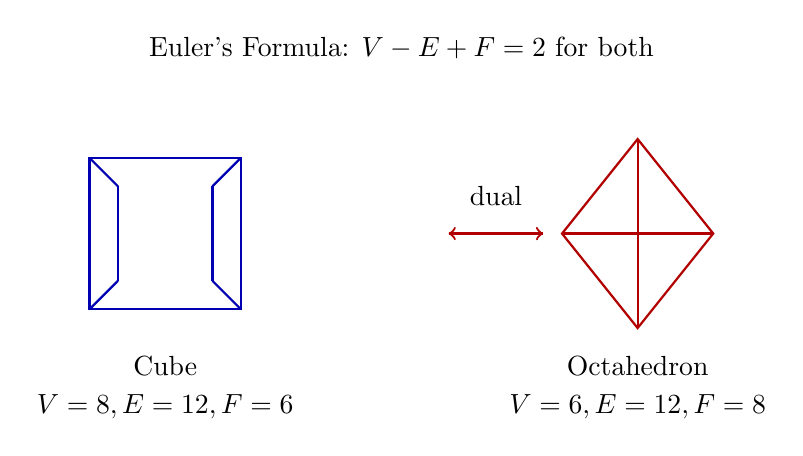
\begin{tikzpicture}[scale=1.2]
  % Cube (left)
  \begin{scope}[shift={(-2.5,0)}]
    \draw[blue!70!black, thick] (-0.8,-0.8) rectangle (0.8,0.8);
    \draw[blue!70!black, thick] (-0.5,-0.5) -- (-0.8,-0.8);
    \draw[blue!70!black, thick] (0.5,-0.5) -- (0.8,-0.8);
    \draw[blue!70!black, thick] (-0.5,0.5) -- (-0.8,0.8);
    \draw[blue!70!black, thick] (0.5,0.5) -- (0.8,0.8);
    \draw[blue!70!black, thick] (-0.5,-0.5) -- (-0.5,0.5);
    \draw[blue!70!black, thick] (0.5,-0.5) -- (0.5,0.5);
    \node[below] at (0,-1.2) {Cube};
    \node[below] at (0,-1.6) {$V=8, E=12, F=6$};
  \end{scope}
  
  % Arrow
  \draw[->, thick, red!70!black] (0.5,0) -- (1.5,0);
  \node at (1,0.4) {dual};
  \draw[->, thick, red!70!black] (1.5,0) -- (0.5,0);
  
  % Octahedron (right)
  \begin{scope}[shift={(2.5,0)}]
    \draw[red!70!black, thick] (0,-1) -- (0.8,0) -- (0,1) -- (-0.8,0) -- cycle;
    \draw[red!70!black, thick] (0,0) -- (0,-1);
    \draw[red!70!black, thick] (0,0) -- (0,1);
    \draw[red!70!black, thick] (0,0) -- (0.8,0);
    \draw[red!70!black, thick] (0,0) -- (-0.8,0);
    \node[below] at (0,-1.2) {Octahedron};
    \node[below] at (0,-1.6) {$V=6, E=12, F=8$};
  \end{scope}
  
  % Title
  \node[above=0.3cm] at (0,1.5) {Euler's Formula: $V - E + F = 2$ for both};
\end{tikzpicture}
